% Created 2018-11-15 Thu 21:34
% Intended LaTeX compiler: pdflatex
\documentclass[presentation]{beamer}
\usepackage[utf8]{inputenc}
\usepackage[T1]{fontenc}
\usepackage{graphicx}
\usepackage{grffile}
\usepackage{longtable}
\usepackage{wrapfig}
\usepackage{rotating}
\usepackage[normalem]{ulem}
\usepackage{amsmath}
\usepackage{textcomp}
\usepackage{amssymb}
\usepackage{capt-of}
\usepackage{natbib}
\usepackage[linktocpage,pdfstartview=FitH,colorlinks,
linkcolor=blue,anchorcolor=blue,
citecolor=blue,filecolor=blue,menucolor=blue,urlcolor=blue]{hyperref}
\setbeamertemplate{frame footer}{\insertshortauthor}
\setbeamerfont{page number in head/foot}{size=\tiny}
\setbeamercolor{footline}{fg=gray}
\usepackage{amsmath}
\author{Florian Hollenbach}
\usepackage[english]{isodate}
\usepackage{amsmath,amsthm,amssymb,amsfonts}
\newcommand{\E}{\mathbb{E}}
\newcommand{\V}{\mathbb{V}}
\usetheme{metropolis}
\usecolortheme{}
\usefonttheme{}
\useinnertheme{}
\useoutertheme{}
\author{Florian Hollenbach}
\date{\today}
\title{Political Science 209 - Fall 2018}
\subtitle{Uncertainty}

\hypersetup{
 pdfauthor={Florian Hollenbach},
 pdftitle={Political Science 209 - Fall 2018},
 pdfkeywords={},
 pdfsubject={},
 pdfcreator={Emacs 25.3.1 (Org mode 9.1.14)}, 
 pdflang={English}}
\begin{document}

\maketitle


\begin{frame}[label={sec:org5f660ea}]{Random Variables and Probability Distributions}
\begin{itemize}
\item What is a random variable? We assigns a number to an event
\begin{itemize}
\item coin flip: tail= 0; heads= 1
\item Senate election: Ted Cruz= 0; Beto O'Rourke= 1
\item Voting: vote = 1; not vote = 0
\end{itemize}
\end{itemize}



\pause

Probability distribution: Probability of an event that a random variable takes a certain value
\end{frame}


\begin{frame}[label={sec:orgedf0a05}]{Random Variables and Probability Distributions}
\begin{itemize}
\item P(coin =1); P(coin = 0)
\item P(election = 1); P(election = 0)
\end{itemize}
\end{frame}


\begin{frame}[label={sec:org7a40ade}]{Random Variables and Probability Distributions}
\begin{itemize}
\item \alert{Probability density function (PDF)}: f(x) How likely does X take a particular value?
\item \alert{Probability mass function (PMF)}: When X is discrete, f(x)=P(X =x)
\end{itemize}

\pause

\begin{itemize}
\item \alert{Cumulative distribution function (CDF)}: F(x) = P(X \(\leq\) x)
\begin{itemize}
\item What is the probability that a random variable X takes a value equal to or less than x?
\item Area under the density curve (either we use the sum \(\Sigma\) or integral \(\int\))
\item Non-decreasing
\end{itemize}
\end{itemize}
\end{frame}


\begin{frame}[fragile,label={sec:org7ef6b24}]{Random Variables and Probability Distributions: Binomial Distribution}
 \begin{itemize}
\item \alert{PMF}: for \(x \in \{0, 1, \dots, n\}\),
\(f(x) \ = \ P(X = x) \ = \ {n \choose x} p^x (1-p)^{n-x}\)

\item \alert{PMF} function to tell us: what is the probability of x \emph{successes} given n trials with with P(x) = p
\end{itemize}

\pause

In \emph{R}:
\begin{verbatim}
dbinom(x = 2, size = 4, prob = 0.1) ## prob of 2 successes in 4 trials with p =0.1
\end{verbatim}

\begin{verbatim}
[1] 0.0486
\end{verbatim}
\end{frame}




\begin{frame}[fragile,label={sec:orgefdd2c4}]{Random Variables and Probability Distributions: Binomial Distribution}
 \begin{itemize}
\item \alert{CDF}: for \(x \in \{0, 1, \dots, n\}\)
\(F(x) \ = \ P(X \le x) \ = \ \sum_{k = 0}^x {n\choose k} p^k (1-p)^{n-k}\)

\item \alert{CDF} function to tell us: what is the probability of \emph{x or fewer} \emph{successes} given n trials with with P(x) = p
\end{itemize}

\pause

In \emph{R}:
\begin{verbatim}
pbinom(2, size = 4, prob = 0.1) ## prob of 2 or fewer successes in 4 trials with p =0.1
\end{verbatim}

\begin{verbatim}
[1] 0.9963
\end{verbatim}
\end{frame}

\begin{frame}[fragile,label={sec:org7e89944}]{PMF and CDF}
 CDF of F(x) is equal to the sum of the results from calculating the PMF for all values smaller and equal to x

\pause


In \emph{R}:
\begin{verbatim}
pbinom(2, size = 4, prob = 0.1) ## CDF

sum(dbinom(c(0,1,2),4,0.1)) ## summing up the pdfs
\end{verbatim}

\begin{verbatim}
[1] 0.9963

[1] 0.9963
\end{verbatim}
\end{frame}

\begin{frame}[label={sec:org5cebe3d}]{Random Variables and Probability Distributions: Binomial Distribution}
\begin{itemize}
\item Example: flip a fair coin 3 times

\(f(x) \ = \ P(X = x) \ = \ {n \choose x} p^x (1-p)^{n-x}\)

\(f(x) \ = \ P(X = 1) \ = \ {3 \choose 1} 0.5^1 (0.5)^{2} = 3*0.5*0.5^2 = 0.375\)
\end{itemize}
\end{frame}


\begin{frame}[fragile,shrink=35,label={sec:orgb1f5b02}]{Random Variables and Probability Distributions: Binomial Distribution}
 \begin{verbatim}
x <- 0:3
barplot(dbinom(x, size = 3, prob = 0.5), ylim = c(0, 0.4), names.arg = x, xlab = "x",
        ylab = "Density", main = "Probability mass function")
\end{verbatim}
\end{frame}



\begin{frame}[label={sec:org8b91b94}]{Random Variables and Probability Distributions: Binomial Distribution}
\begin{center}
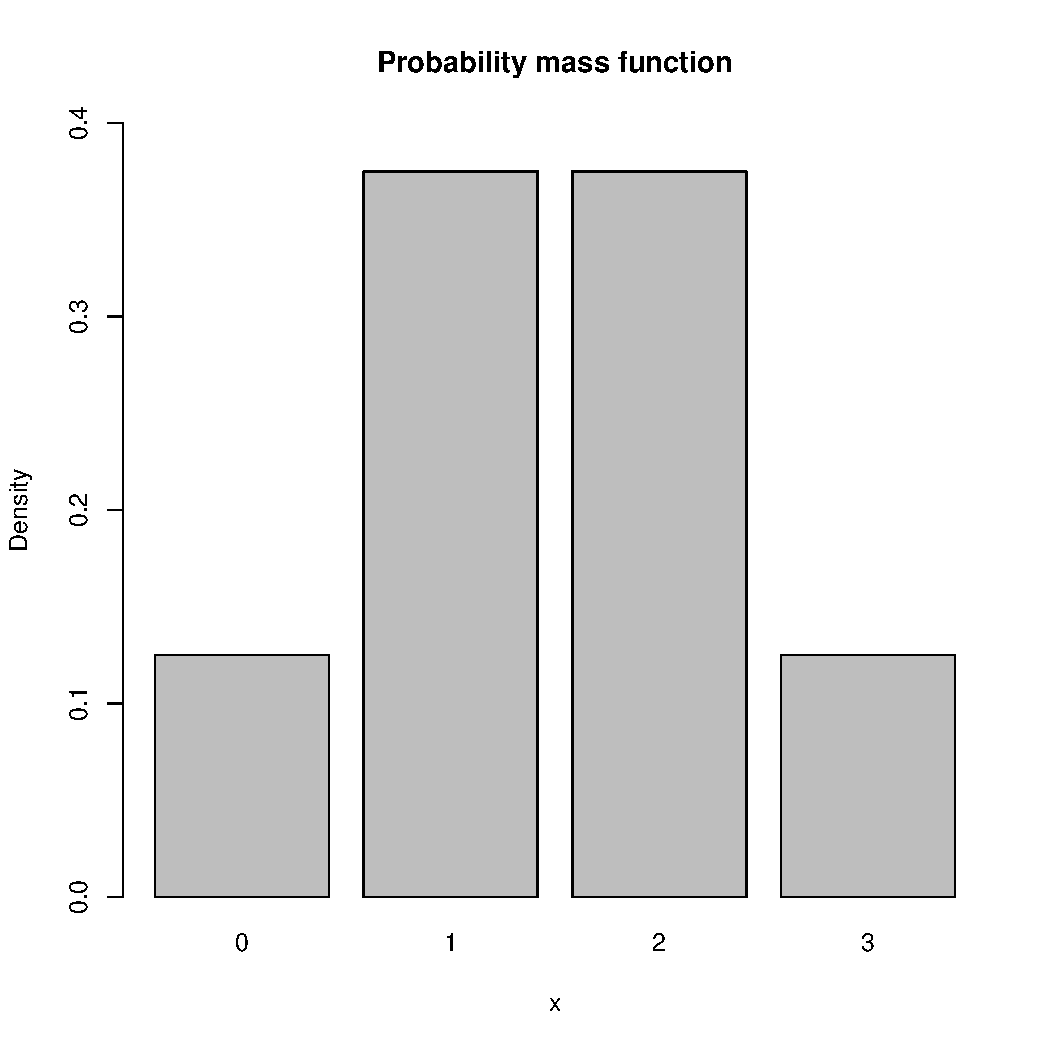
\includegraphics[width=6cm]{/Users/florianhollenbach/Documents/GitHub/Polisci209_2018/slides/week11/barplot.pdf}
\end{center}
\end{frame}


\begin{frame}[fragile,shrink=35,label={sec:org0c12b64}]{Random Variables and Probability Distributions: Binomial Distribution}
 \begin{verbatim}
x <- -1:4
pb <- pbinom(x, size = 3, prob = 0.5)
plot(x[1:2], rep(pb[1], 2), ylim = c(0, 1), type = "s", xlim = c(-1, 4), xlab = "x",
     ylab = "Probability", main = "Cumulative distribution function")
for (i in 2:(length(x)-1)) {
    lines(x[i:(i+1)], rep(pb[i], 2))
}
points(x[2:(length(x)-1)], pb[2:(length(x)-1)], pch = 19)
points(x[2:(length(x)-1)], pb[1:(length(x)-2)])
\end{verbatim}
\end{frame}




\begin{frame}[label={sec:org2c7ac6a}]{Random Variables and Probability Distributions: Binomial Distribution}
\begin{center}
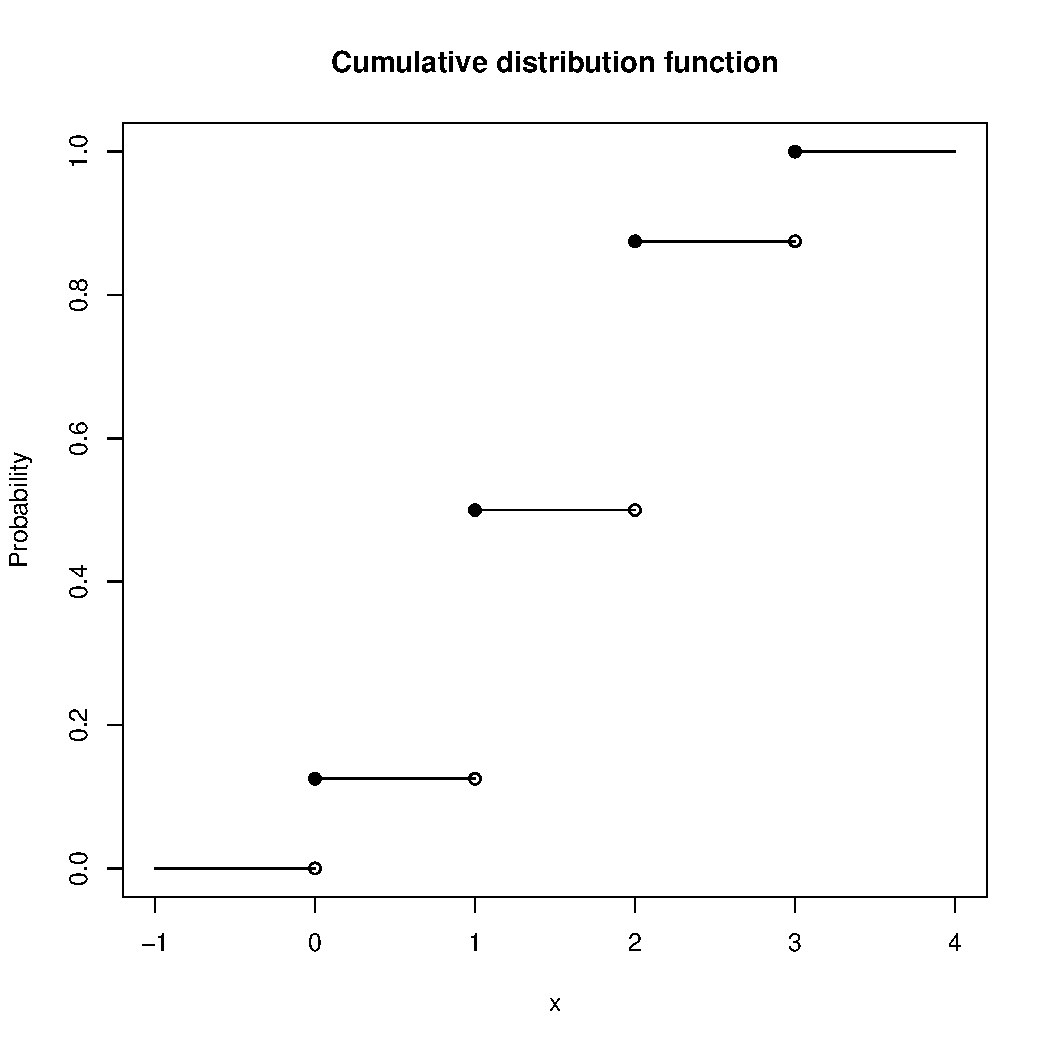
\includegraphics[width=6cm]{/Users/florianhollenbach/Documents/GitHub/Polisci209_2018/slides/week11/cdf_binom.pdf}
\end{center}
\end{frame}



\begin{frame}[label={sec:org1a9a5aa}]{Random Variables and Probability Distributions: Normal Distribution}
\alert{Normal distribution}

\begin{center}
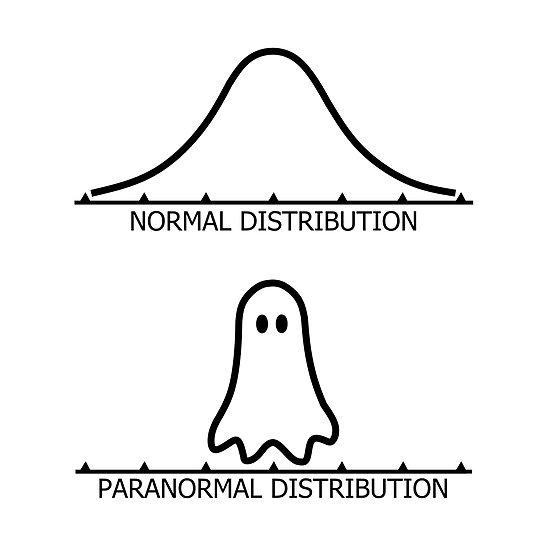
\includegraphics[width=6cm]{/Users/florianhollenbach/Documents/GitHub/Polisci209_2018/slides/week11/paranormal.jpg}
\end{center}
\end{frame}



\begin{frame}[label={sec:org17b3814}]{Random Variables and Probability Distributions: Normal Distribution}
\alert{Normal distribution} also called \alert{Gaussian distribution}



\begin{center}
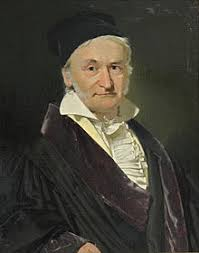
\includegraphics[width=6cm]{/Users/florianhollenbach/Documents/GitHub/Polisci209_2018/slides/week11/gauss.jpeg}
\end{center}
\end{frame}


\begin{frame}[label={sec:org47d6e1e}]{Normal distribution}
\begin{itemize}
\item Takes on values from -\(\infty\) to \(\infty\)
\item Defined by two things: \(\mu\) and \(\sigma^{2}\)
\begin{itemize}
\item Mean and Variance (standard deviation squared)
\end{itemize}
\end{itemize}


\begin{itemize}
\item Mean defines the location of the distribution
\item Variance defines the spread
\end{itemize}
\end{frame}



\begin{frame}[fragile,label={sec:org05219cb}]{Random Variables and Probability Distributions: Normal Distribution}
 \alert{Normal distribution} with mean \(\mu\) and standard deviation \(\sigma\)
\begin{itemize}
\item \alert{PDF}:
\(f(x) \ = \ \frac{1}{\sqrt{2\pi} \sigma}\exp\left(-\frac{(x - \mu)^2}{2\sigma^2}\right)\)
\end{itemize}

\pause


In \emph{R}:
\begin{verbatim}
dnorm(2, mean = 2, sd = 2) ## probability of x =2 with normal variable mean 2 sd 2
\end{verbatim}

\begin{verbatim}
[1] 0.1994711
\end{verbatim}
\end{frame}



\begin{frame}[fragile,label={sec:orgb29ddf5}]{Random Variables and Probability Distributions: Normal Distribution}
 \begin{itemize}
\item \alert{CDF} (no simple formula. use \R{} to compute it):
\(F(x) \ = \ P(X \le x) \ = \ \int_{-\infty}^x
   \frac{1}{\sqrt{2\pi}\sigma}\exp\left(-\frac{(t - \mu)^2}{2\sigma^2}\right) dt\)
\end{itemize}
\begin{itemize}
\item What will be F(x =2) for N(2,4)?
\end{itemize}
\pause

In \emph{R}:
\begin{verbatim}
pnorm(2, mean = 2, sd = 2) ## probability of x =2 with normal variable mean 2 sd 2
\end{verbatim}

\begin{verbatim}
[1] 0.5
\end{verbatim}
\end{frame}


\begin{frame}[label={sec:orgbcf0e7a}]{Normal distribution}
\begin{itemize}
\item Normal distribution is symmetric around the mean
\item Mean = Median
\end{itemize}
\end{frame}





\begin{frame}[label={sec:org03e82cc}]{Random Variables and Probability Distributions: Normal Distribution}
\begin{center}
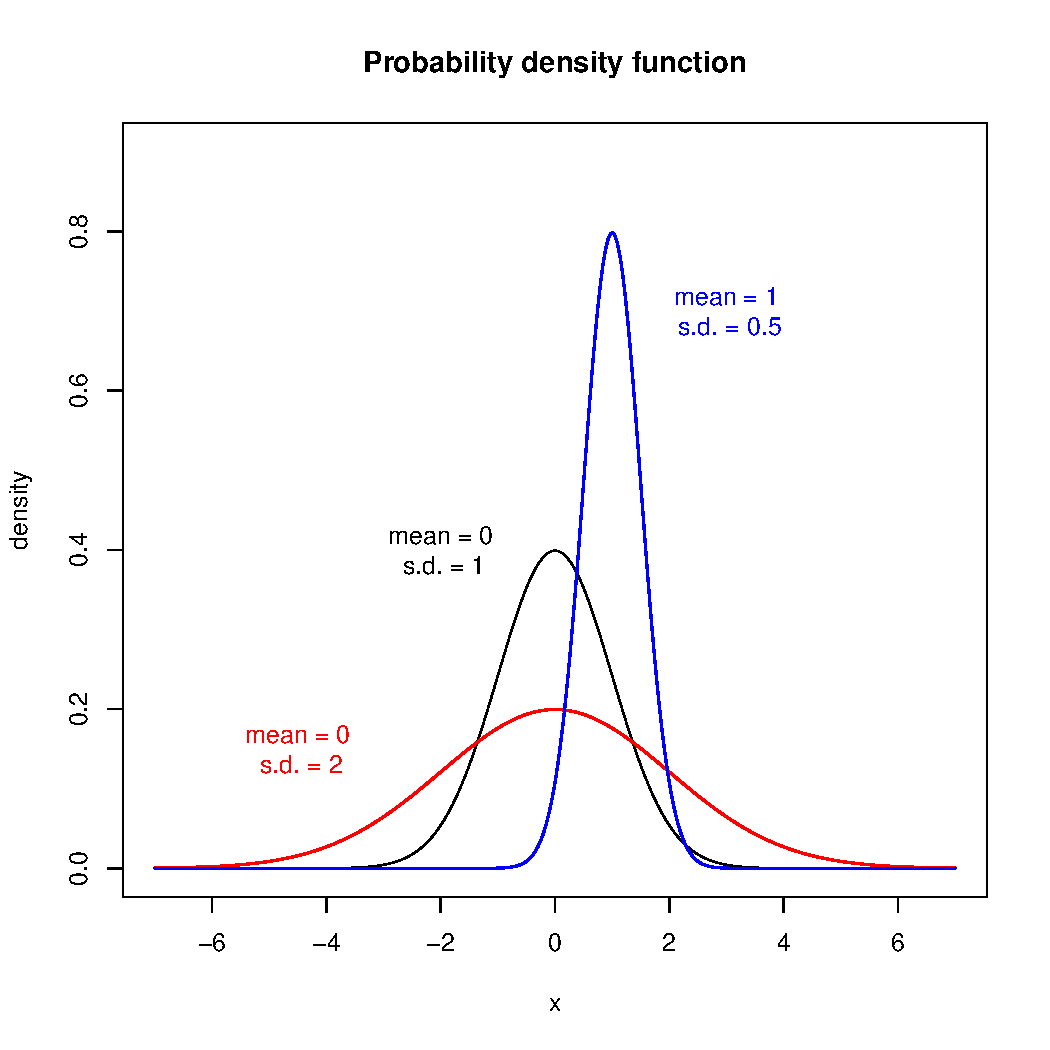
\includegraphics[width=5cm]{/Users/florianhollenbach/Documents/GitHub/Polisci209_2018/slides/week11/normal.pdf}
\end{center}
\end{frame}


\begin{frame}[fragile,shrink=30,label={sec:org8674453}]{Random Variables and Probability Distributions: Normal Distribution in R}
 \begin{verbatim}
x <- seq(from = -7, to = 7, by = 0.01)
plot(x, dnorm(x), xlab = "x", ylab = "density", type = "l",
     main = "Probability density function", ylim = c(0, 0.9))
lines(x, dnorm(x, sd = 2), col = "red", lwd = lwd)
lines(x, dnorm(x, mean = 1, sd = 0.5), col = "blue", lwd = lwd)
\end{verbatim}
\end{frame}


\begin{frame}[label={sec:org34881dd}]{Random Variables and Probability Distributions: Normal Distribution in R}
\begin{center}
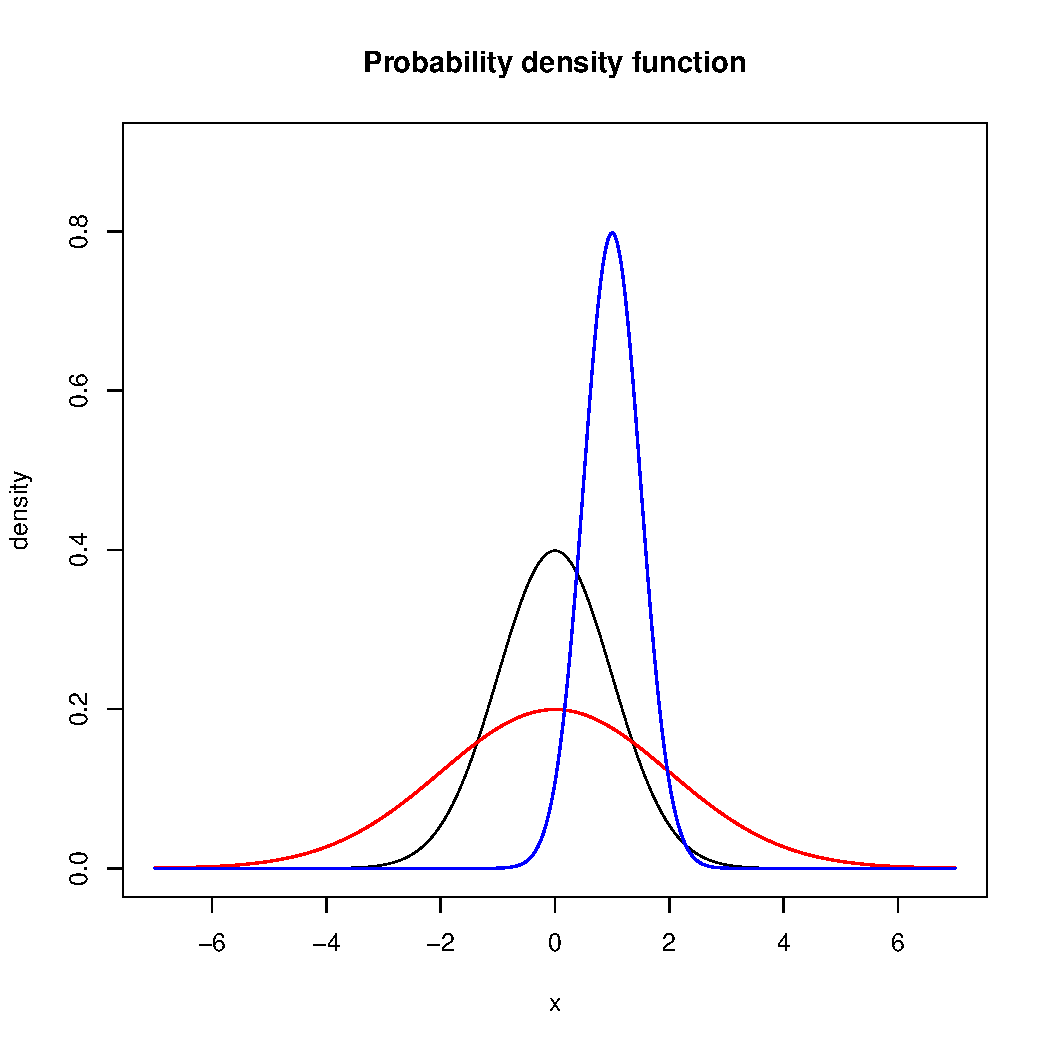
\includegraphics[width=5cm]{/Users/florianhollenbach/Documents/GitHub/Polisci209_2018/slides/week11/normal_pdf.pdf}
\end{center}
\end{frame}


\begin{frame}[fragile,shrink=30,label={sec:orgdfa7e32}]{Random Variables and Probability Distributions: Normal Distribution in R}
 \begin{verbatim}
plot(x, pnorm(x), xlab = "x", ylab = "probability", type = "l",
     main = "Cumulative distribution function", lwd = lwd)
lines(x, pnorm(x, sd = 2), col = "red", lwd = lwd)
lines(x, pnorm(x, mean = 1, sd = 0.5), col = "blue", lwd = lwd)
\end{verbatim}
\end{frame}


\begin{frame}[label={sec:org8151561}]{Random Variables and Probability Distributions: Normal Distribution in R}
\begin{center}
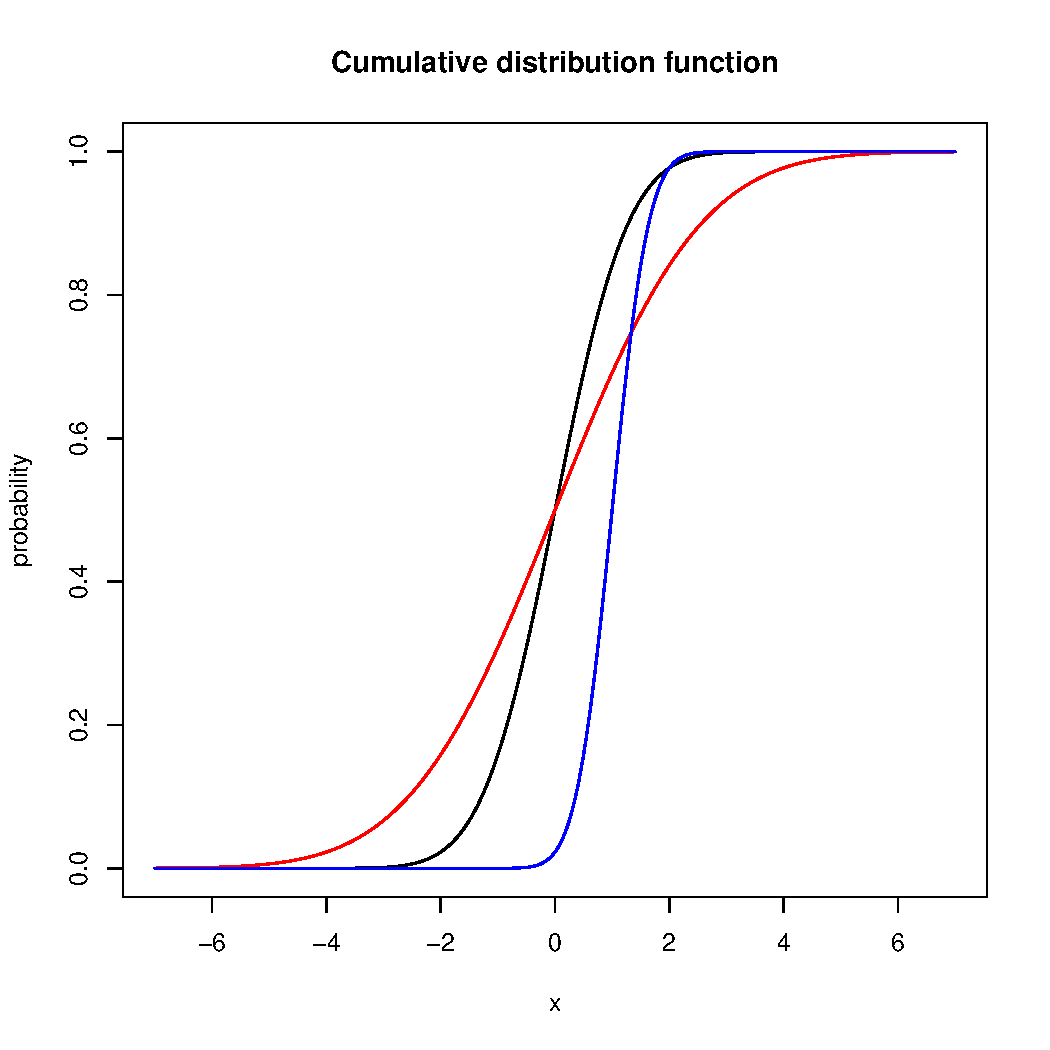
\includegraphics[width=5cm]{/Users/florianhollenbach/Documents/GitHub/Polisci209_2018/slides/week11/normal_cdf.pdf}
\end{center}
\end{frame}


\begin{frame}[label={sec:org0301030}]{Random Variables and Probability Distributions: Normal Distribution}
Let \(X \sim N(\mu,\,\sigma^{2})\), and c be some constant

\begin{itemize}
\item Adding/subtracting to/from a random variable that is normally distributed also results in a variable with a normal distribution:
Z = X + c then \(Z \sim N(\mu +c,\,\sigma^{2})\)
\end{itemize}

\pause


\begin{itemize}
\item Multiplying or dividing a random variable that is normally distributed also results in a variable with a normal distribution:
\(Z = X\times c\) then \(Z  \sim N(\mu \times c,\,(\sigma \times c)^{2})\)

\item Z-score of a random variable that is normally distributed has mean 0 and sd = 1
\end{itemize}
\end{frame}


\begin{frame}[label={sec:orgde8f89c}]{Random Variables and Probability Distributions: Normal Distribution}
Curve of the standard normal distribution:

\begin{itemize}
\item Symmetric around 0
\item Total area under the curve is 100\%
\item Area between -1 and 1 is \textasciitilde{}68\%
\item Area between -2 and 2 is \textasciitilde{}95\%
\item Area between -3 and 3 is \textasciitilde{}99.7\%
\end{itemize}
\end{frame}

\begin{frame}[fragile,shrink=30,label={sec:orgfbb04d7}]{Random Variables and Probability Distributions: Normal Distribution}
 \begin{verbatim}
x <- seq(from = -7, to = 7, by = 0.01)
lwd <- 1.5
plot(x, dnorm(x), xlab = "x", ylab = "density", type = "l",
     main = "Probability density function", ylim = c(0, 0.9))
abline(v= -1, col = "red")
abline(v= 1, col = "red")
abline(v= -2, col = "green")
abline(v= 2, col = "green")
\end{verbatim}
\end{frame}



\begin{frame}[label={sec:org307ef66}]{Random Variables and Probability Distributions: Normal Distribution}
\begin{center}
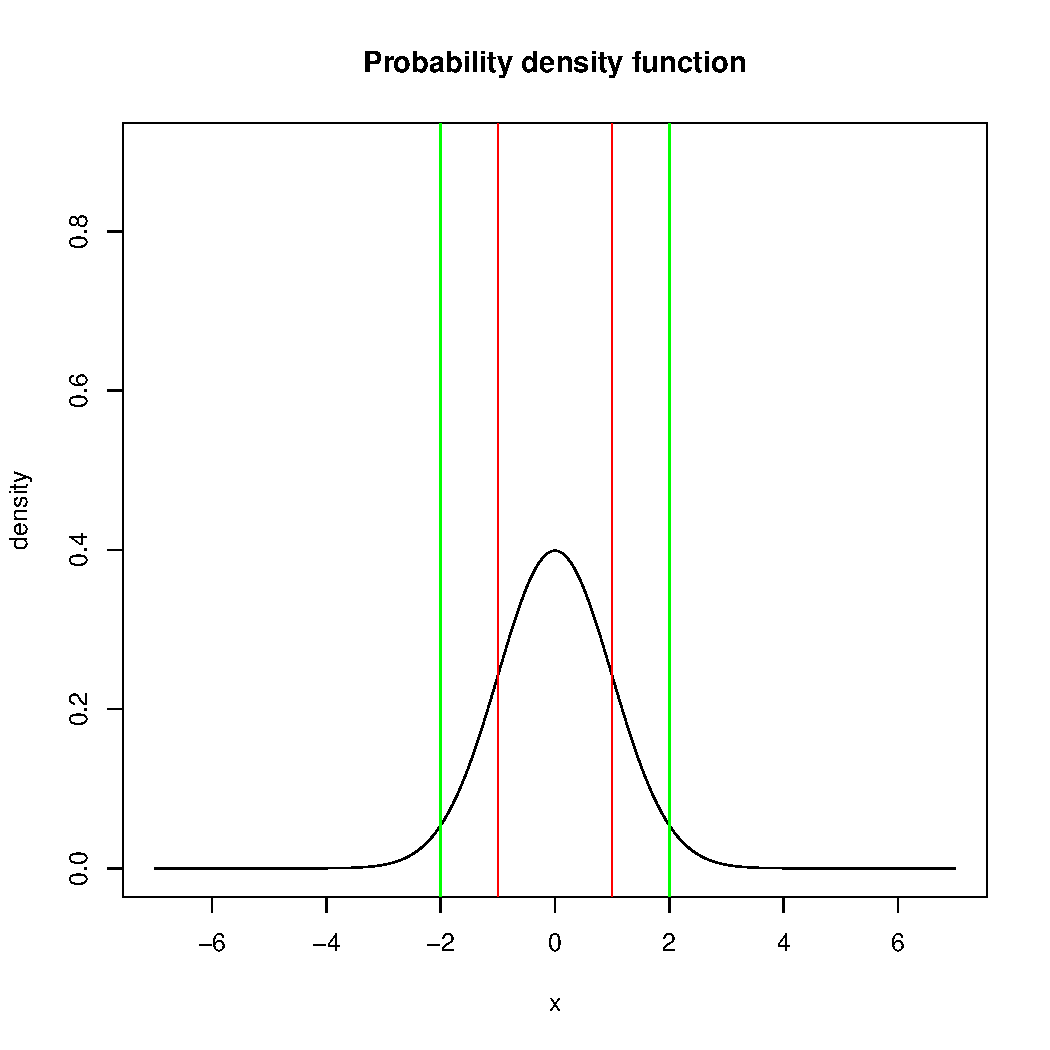
\includegraphics[width=7cm]{/Users/florianhollenbach/Documents/GitHub/Polisci209_2018/slides/week11/normal_example.pdf}
\end{center}
\end{frame}


\begin{frame}[label={sec:org8f8d974}]{Random Variables and Probability Distributions: Normal Distribution}
Curve of the \alert{any} normal distribution:

\begin{itemize}
\item Symmetric around mean
\item Total area under the curve is 100\%
\item Area between -1SD and +1SD is \textasciitilde{}68\%
\item Area between -2SD and +2SD is \textasciitilde{}95\%
\item Area between -3SD and +3SD is \textasciitilde{}99.7\%
\end{itemize}
\end{frame}


\begin{frame}[label={sec:org2c3b447}]{Random Variables}
\emph{Expectations}, \emph{Means}, and \emph{Variances}

For probability distributions, means should not be confused with \emph{sample means}

Expectations or means of a random variable have specific meanings for its the probability distribution
\end{frame}


\begin{frame}[label={sec:org3e3fc86}]{Means and Expectation}
A sample mean varies from sample to sample

Mean of a probability distribution is a theoretical construct and constant

\pause

Example: Age of undergraduate body at A\&M
\end{frame}

\begin{frame}[label={sec:org7d52123}]{Means and Expectation}
The expectation of a random variable is equal to the sum of all possibilities \emph{weighted} by the probabilities

\pause

Example: expectation of rolling one die

\(\E(X)\) = \(\frac{1}{6} \times 1 + \frac{1}{6} \times 2 + \frac{1}{6} \times 3 + \frac{1}{6} \times 4 \frac{1}{6} \times 5 \frac{1}{6} \times 6 = 3.5\)
\end{frame}



\begin{frame}[label={sec:orgc511f9b}]{Means and Expectation}
The expectation of a random variable is equal to the sum of all possibilities \emph{weighted} by the probabilities

\begin{equation*}
     \E(X) \ = \ \left\{\begin{array}{ll}
                          \sum_{x} x\ f(x)
                          & \textsf{if } X \ \textsf{is discrete} \\
                          \int x\ f(x) dx & \textsf{if } X \ \textsf{is continuous}
                        \end{array}\right.
\end{equation*}
\end{frame}

\begin{frame}[label={sec:org42917ab}]{Means and Expectation}
Remember the lottery!

Expected value: winnings \(\times\) p(winning) + 0 \(\times\) p(not winning)
\end{frame}


\begin{frame}[label={sec:orgd59f084}]{Means and Expectation}
What is \(\E(X)\) for the number of heads in 100 coin flips?

\pause

\(\E(X) = 0.5\times 1 + 0.5\times 1+ ... + 0.5\times 1 = 0.5*100 = 50\)
\end{frame}

\begin{frame}[label={sec:orgdc33274}]{Variance}
\begin{itemize}
\item Variance is standard deviation squared

\item Variance in a probability distribution indicates how much uncertainty exists

\item Similar \alert{but not the same} as sample standard deviation
\end{itemize}
\end{frame}

\begin{frame}[label={sec:orgb1bd9cc}]{Variance}
Population variance: \(\V(X) \ = \ \E[\{X - \E(X)\}^2] \ = \ \E(X^2) - \{\E(X)\}^2\)
\end{frame}
\end{document}